\documentclass[12pt,spanish]{article}
\usepackage[spanish,activeacute]{babel}
\renewcommand\shorthandsspanish{}
\usepackage[utf8]{inputenc}
\usepackage{fancyhdr,a4wide,enumerate}
\usepackage{lastpage}
\usepackage{caratula}
\usepackage{float}
\usepackage{graphicx}
\usepackage{amsthm,amsmath,pxfonts,amssymb}
\usepackage[linesnumbered,ruled]{algorithm2e}

\setlength{\headheight}{16pt}
\pagestyle{fancy}
\lhead{Trabajo Práctico D}
\rhead{Eugenio Costa, Emiliano González, Lisandro Sebrié}
\cfoot{\thepage\ de \pageref{LastPage}}
\renewcommand{\headrulewidth}{0.4pt}
\renewcommand{\footrulewidth}{0.4pt}

\theoremstyle{plain}
\newtheorem*{theorem}{Teorema}
\newtheorem*{lemma}{Lema}
\newtheorem*{proposition}{Proposición}
\newtheorem*{corollary}{Corolario}

\theoremstyle{definition}
\newtheorem*{definition}{Definición}

\dontprintsemicolon
\linesnumberedhidden
\nocaptionofalgo
\SetKwIF{If}{ElseIf}{Else}{si}{luego}{sino si}{sino}{fin si}
\SetKw{Return}{devolver}
\SetKwFor{For}{para}{hacer}{fin para}
\SetKwFor{ForEach}{para cada}{hacer}{fin para}
\SetKwFor{ForAll}{repetir}{veces}{fin repetir}
\SetKwFor{While}{mientras}{hacer}{fin mientras}
\SetKwFor{Rep}{repetir}{veces}{fin repetir}
\SetKwRepeat{Repeat}{repetir}{hasta que}
\SetKw{KwTo}{hasta}
\SetKwInOut{Input}{entrada}
\SetKwInOut{Output}{salida}

\DeclareMathOperator{\set}{set}
\DeclareMathOperator{\sgn}{sgn}
\newcommand{\nat}{\mathbb{N}}
\newcommand{\integ}{\mathbb{Z}}

\begin{document}

\materia{Problemas, Algoritmos y Programación}
\titulo{Trabajo Práctico D}
\grupo{Grupo 14}
\integrante{Eugenio Costa}{839/06}{tutecosta@gmail.com}
\integrante{Emiliano González}{426/06}{xjesse\_jamesx@hotmail.com}
\integrante{Lisandro Sebrié}{358/03}{lsebrie@hotmail.com}

\maketitle

\newpage
\section*{10625 -- ``GNU = GNU'sNotUnix''}
\subsection*{Problema y solución}

El objetivo de este problema es simular reemplazos de caracteres en un
string, y calcular la cantidad de apariciones de un caracter determinado
en la cadena transformada. Los datos de entrada son las reglas $Q_i$ a aplicar,
un string $s$ que define la frecuencia inicial de cada caracter, el número de
veces $n$ a aplicar las reglas y el caracter $c$ del que se desea conocer su
frecuencia.

Por obvias razones de eficiencia no ejecutamos los reemplazos sobre el
string dado, sino que los simulamos guardando en una matriz la frecuencia
de cada caracter. Esta matriz contiene inicialmente las frecuencias con
que aporta cada caracter según las reglas, y tiene la propiedad de que,
al multiplicarla por sí misma (con algunos cuidados, detallados en la sección
sobre implementación) mantiene las frecuencias de haber aplicado una vez las
reglas dadas sobre el string.

Así, para el caso de ejemplo $A \rightarrow BAcX$, y dado el string de inicio
$ABCcXA$, ejemplos de matriz serán:

$$M =
\begin{array}{l}
\begin{matrix}
	\ \ A & B & C & X & c
\end{matrix} \\
\left(
	\begin{array}{ccccc}
	1 & 1 & 0 & 1 & 1 \\
	0 & 0 & 0 & 0 & 0 \\
	0 & 0 & 0 & 0 & 0 \\
	0 & 0 & 0 & 0 & 0 \\
	0 & 0 & 0 & 0 & 0 \\
	\end{array}
\right)
\hspace{1cm}
M^2 = \left(
\begin{array}{ccccc}
1 & 2 & 0 & 2 & 2 \\
0 & 0 & 0 & 0 & 0 \\
0 & 0 & 0 & 0 & 0 \\
0 & 0 & 0 & 0 & 0 \\
0 & 0 & 0 & 0 & 0 \\
\end{array}
\right)
\hspace{1cm}
M^3 = \left(
\begin{array}{ccccc}
1 & 3 & 0 & 3 & 3 \\
0 & 0 & 0 & 0 & 0 \\
0 & 0 & 0 & 0 & 0 \\
0 & 0 & 0 & 0 & 0 \\
0 & 0 & 0 & 0 & 0 \\
\end{array}
\right)
\end{array}
$$

Cada valor $M_{ij}^k$ representa la cantidad de caracteres $`j'$ que incorpora
el caracter $`i'$ en la $k$-ésima aplicación de reglas. La frecuencia
de un caracter $c$ luego de $n$ aplicaciones de reglas sobre una cadena $str$
(la respuesta al problema) resulta ser:
$$\sum_i M_{ic}^n \times cant\_apariciones(str, c)$$


\subsection*{Detalles de Implementación}

Si hay caracteres en el string que no dan inicio a reglas, algunas filas de
la matriz quedarán nulas, lo que puede redundar en pérdidas de información al
hacer las multiplicaciones. Es fácil ver, en el ejemplo anterior, que $M=M^n\
\forall\ n$. Dado que el enunciado indica que todo caracter que no aparece en
una regla se mantiene, podría mantenerse la diagonal en 1 como implementación
de dicha identidad. Pero por la forma en que calculamos la frecuencia nos fue
conveniente modificar levemente la multiplicación de matrices para que
mantenga los datos necesarios. Procedemos de la siguiente manera: antes de
reemplazar el valor de $M_{ij}$ chequeamos si $j$ es un caracter que da
inicio a reglas (mediante el vector {\tt in\_queries}). En ese caso, se
reemplaza $M_{ij}$ normalmente y se continúa la multiplicación; en caso
contrario, en lugar de reemplazarlo, se suma el nuevo valor al que contenía
dicha celda. De esta manera se lleva cuenta del agregado de caracteres aunque
la fila correspondiente sea nula.

Dado que los valores se encuentran entre los números 33 y 126 de la tabla ASCII,
armamos matrices de dimensión $94\times 94$, que representan a todos los valores
de entrada posibles. Al direccionar caracteres en la matriz restamos un {\sl offset}
de 33 a su valor ASCII.

Utilizamos el tipo de datos {\tt unsigned long long int} para las matrices y
el valor de frecuencia.


\subsection*{Análisis de complejidad}

Para calcular $M^e$ utilizamos el algoritmo de exponenciación binaria, basado en
que $x^e = (x^\frac e 2)^2$ (si $e$ es par), disminuyendo la cantidad de
multiplicaciones en forma logarítmica respecto del valor del exponente. Así, la
multiplicación de matrices (algoritmo de orden $N^3$, siendo $N$
la cantidad de columnas) se ejecuta $O(\log e)$ veces.

Rellenar la matriz con las $N$ {\sl queries} toma $O(N^3)$, y calcular la suma
final de frecuencias toma $O(N)$, por lo que la complejidad total resulta de
$O(N^3\log e + N)$.

\newpage
\section*{3928 -- ``Ballroom Lights''}
\subsection*{Problema y modelo}
El problema trata sobre un salón de exposiciones que cuenta con una cantidad dada de
bombillas de luz (se supone que la única fuente de luz es esta) que son fuentes de
luz puntual, y una cantidad dada de columnas, que están ubicadas de forma que no
intersecan la pared ni entre ellas, pero sí pueden tocarse. Las bombillas de luz están
ubicadas de forma que no tocan ninguna columna ni la pared. El escenario se presenta
en dos dimensiones, visto desde arriba (desde el techo del salón). Dado un salón como
el descripto, queremos saber cuál es el perímetro de la pared que cuenta con iluminación.
Se supone que la sombra no sufre difusión ni hay fenómenos reflexión de luces.

Representamos la bombilla como un punto $(x,y)$ en el plano, las columnas como circulos
$(x,y,r)$ de centro $(x,y)$ y radio $r$, y las paredes como 4 segmentos: $\overline{AB}$,
$\overline{BC}$, $\overline{CD}$, $\overline{DA}$, siendo

\vspace{0.2cm}
$A = (0, 0)$

$B = (X, 0)$

$C = (X, Y)$

$D = (0, Y)$
\vspace{0.2cm}

con X e Y dados por el enunciado, por ejemplo:

\begin{figure}[H]
\centering
\label{bl_1}
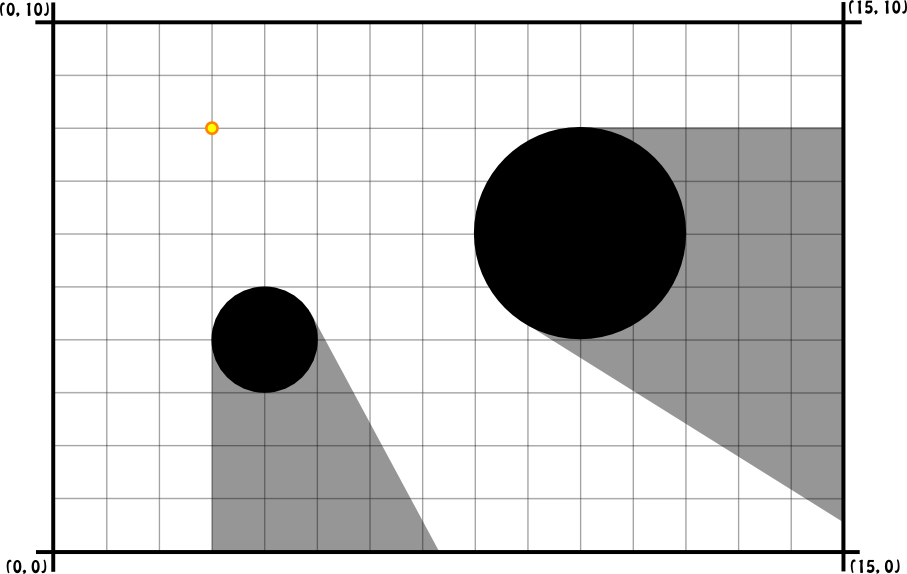
\includegraphics[scale=1.0]{./figuras/bl_1.png}
\caption{Ejemplo del modelo}
\end{figure} 

\subsection*{Solución}

Como dice el enunciado, un punto $p$ dado del perímetro de la pared es iluminado si
existe un segmento de línea (un rayo de luz) que comienza en una bombilla de luz, finaliza
en p y no toca o pasa a través de alguna columna, por lo tanto:
\begin{itemize}
\item Una cierta porción de la pared está iluminada si alguna bombilla la ilumina (por lo tanto
no está iluminada si ninguna bombilla la ilumina, es decir, si todas las columnas proyectan una
sombra sobre esta parte de la pared).
\item La sombra que proyecta una columna $c$ a partir de la luz que incide una bombilla $b$
depende de las tangentes del círculo (que representa la columna $c$) que pasan por el punto
$b$, de forma que, detrás de la columna (visto desde la bombilla) desde una
tangente a la otra se proyectará sombra (si ninguna otra bombilla ilumina la porción) y todo
lo demás se iluminará (si la luz no cruza ninguna otra columna).
\end{itemize}

La solución que presentamos aprobecha estas características. La idea básica del algoritmo es
tomar cada luz y para cada una de ellas calcular las porciones de pared que ilumina.
Para esto recorremos todas las columnas y calculamos la sombra que genera la luz con cada columna
usando las tangentes de la columna que pasan por el punto que representa la luz,
y con estas sombras generamos un conjunto de sombras para cada luz.

Para describir el conjunto de sombras vemos la pared como un único intervalo $(0, 2X + 2Y)$, como
si estuviésemos recorriendo las paredes en sentido antihorario, comenzando desde la pared inferior,
por ejemplo:

\begin{figure}[H]
\centering
\label{bl_2}
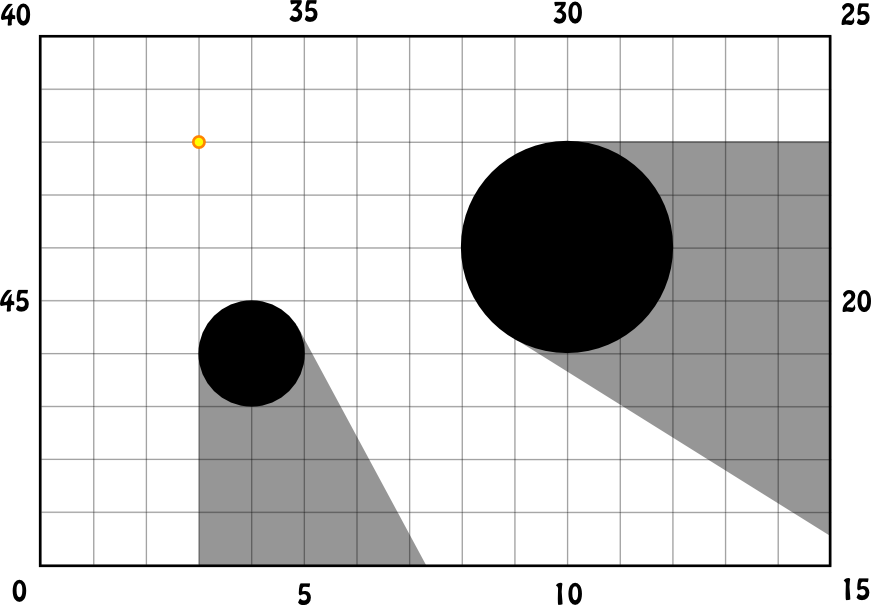
\includegraphics[scale=1.0]{./figuras/bl_2.png}
\caption{Pared vista como un intervalo en R}
\end{figure}

y las sombras como subintervalos del mismo (para ver cómo se hace esta traducción de los segmentos
de pared a un intervalo ir a la sección de Cálculo de sombras).
El complemento de un conjunto de sombras son los intervalos de pared iluminada, y resulta simple
de calcular si antes nos aseguramos que para este conjunto de intervalos todos sus elementos tengan
intersección vacía. Para esto ``comprimimos'' el conjunto (realizamos la union entre intervalos de
intersección no vacía) y luego su complemento.

A continuación unimos todos los conjuntos de intervalos iluminados por las bombillas, formando
otro conjunto. Nuevamente, es simple calcular la longitud de las porciones iluminadas del salón
si nos aseguramos que para este conjunto todos sus elementos tengan intersección vacía. Para esto
``comprimimos'' el conjunto en el mismo sentido que antes y calculamos el resultado del problema,
que es:

\vspace{0.2cm}
\begin{center}$\displaystyle\sum_{e \in intIlum}e_y - e_x$\end{center}
\vspace{0.2cm}

Notar que $(\forall e \in intIlum)e_y > e_x$, por construcción (ver la sección de
Cálculo de sombras).

Para contemplar el error de las operaciones entre flotantes utilizamos un $\epsilon = 0.0000001$, 
de modo que dos flotantes $x_1$ y $x_2$ son considerados iguales si: $abs(x_1 - x_2) < \epsilon$.

\subsection*{Cálculo de sombras}
Dada una luz $L = (l_x, l_y)$ y una columna $C = (c_x, c_y, c_r)$ para calcular la porción sobre
la que se proyecta una sombra consideramos los triángulos que se forman como muestra el siguiente
gráfico:

\begin{figure}[H]
\centering
\label{bl_3}
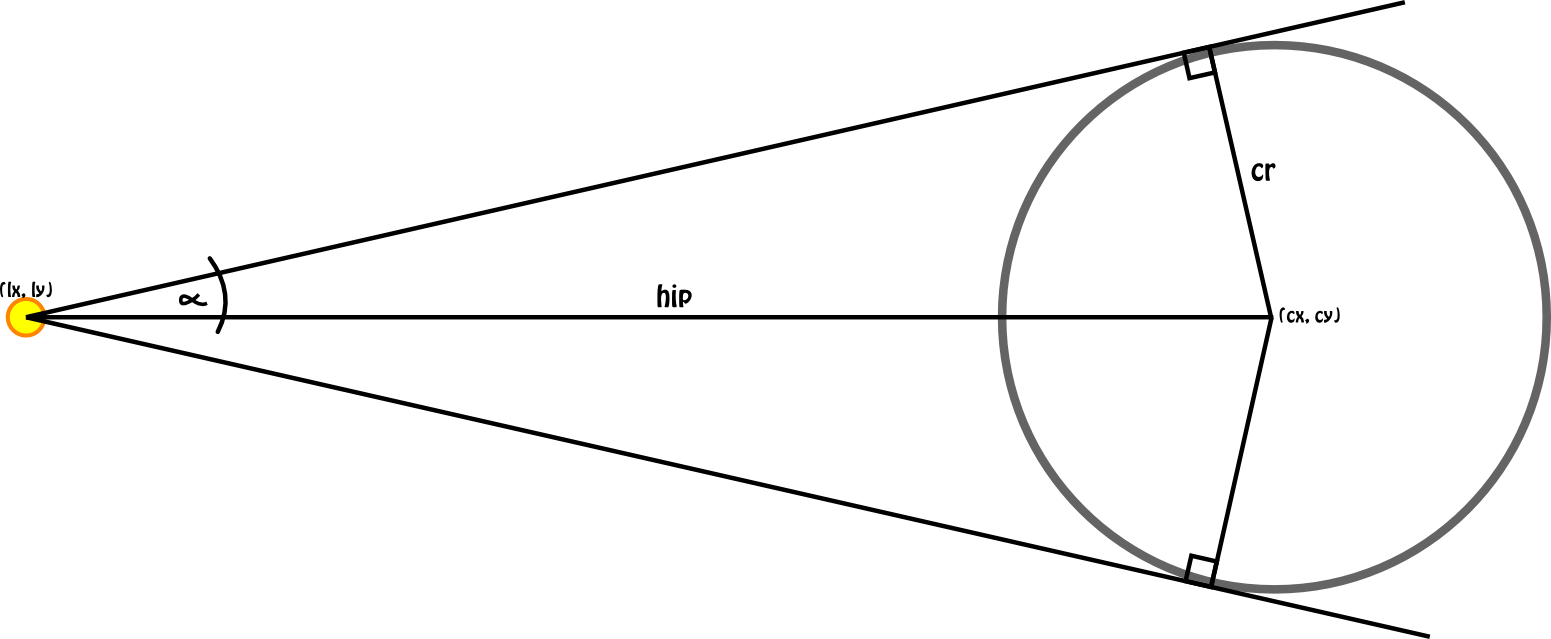
\includegraphics[scale=1.0]{./figuras/bl_3.png}
\caption{los rayos de luz que inciden en la columna}
\end{figure} 

y con esto:

\begin{itemize}
\item calculamos el vector $v = (c_x - l_x, c_y - l_y)$ que es el que va desde la luz hacia
el centro de la columna.
\item el largo de la hipotenusa coincide con la norma del vector $v$, por lo tanto calculamos $|v|$.
\item dado que son triángulos rectángulos, calculamos el seno de alfa como
$\displaystyle\frac{c_r}{hip}$ por trigonometría.
\item por la propiedad $\sin^2(\alpha) + \cos^2(\alpha) = 1$, despejamos y calculamos $\cos(\alpha)$
\item \textbf{calculamos las tangentes:} rotamos el vector $v$ un ángulo $\alpha$ y un ángulo
$-\alpha$, teniendo en cuenta las propiedades $\sin(-\alpha) = -\sin(\alpha)$ y
$\cos(-\alpha) = \cos(\alpha)$, multiplicando:

\vspace{0.2cm}
\begin{center}
$\left(
\begin{array}{cc}
\cos(\alpha) & -\sin(\alpha) \\
\sin(\alpha) & \cos(\alpha) \\
\end{array}
\right)
v = t_1$
\hspace{1cm}
$\left(
\begin{array}{cc}
\cos(\alpha) & \sin(\alpha) \\
-\sin(\alpha) & \cos(\alpha) \\
\end{array}
\right)  
v = t_2$
\end{center}
\vspace{0.2cm}

esto resulta en dos vectores $t_1$ y $t_2$. A partir de estos vectores consideramos las semirrectas
$st_1$ y $st_2$, ambas de origen $(l_x, l_y)$ y con vectores generadores $t_1$ y $t_2$
respectivamente. Las semirrectas las representamos en su forma vectorial.
\item \textbf{calculamos los puntos de intersección $(x_1, y_1)$ y $(x_2, y_2)$ de las semirrectas
$st_1$ y $st_2$ respectivamente con los segmentos que representan la pared:} ver sección
``Intersección entre semirrecta y segmento''.
\item \textbf{a partir de los puntos de intersección calculamos el intervalo de sombra}
considerando los 4 segmentos de la pared como un único segmento del largo del perímetro,
de la siguiente forma:

sea la función de $R^2 \times R$

\vspace{0.2cm}
\begin{center}
\[ f(x, y) = \left\{
               \begin{array}{llll}
				 $x$ & \mbox{si $0 \le x < X \wedge y = 0$} \\
				 $X + y$ & \mbox{si $x = X \wedge 0 \le y < Y$} \\
				 $2X + Y - x$ & \mbox{si $0 < x \le X \wedge y = Y$} \\
				 $2X + 2Y - y$ & \mbox{si $x = 0 \wedge 0 < y \le Y$}
			   \end{array}
			 \right.
\]
\end{center}
\vspace{0.2cm}

\end{itemize}

entonces el intervalo de sombra lo definimos como $(f(x_1,y_1), f(x_2,y_2))$ si
$f(x_1,y_1) \le f(x_2,y_2)$, sino definimos la sombra con dos intervalos: $(0, f(x_2,y_2))$ y
$(f(x_1,y_1), 2X + 2Y)$. Este último caso sucede cuando está el punto $(0,0)$ entre las 
semirrectas tangentes a la columna.

\subsection*{Intersección entre semirrecta y segmento}

Dada una semirrecta de origen $(x_1, y_1)$ y vector generador $(x_2 - x_1, y_2 - y_1)$ y un
segmento $<(w_1, z_1), (w_2, z_2)>$:
\begin{itemize}
\item construímos, con el segmento, una semirrecta de origen $(w_1, z_1)$ y vector generador
$(w_2 - w_1, z_2 - z_1)$.
\item calculamos la intersección entre estas semirrectas, y para esto hacemos el mismo cálculo que
para las rectas, y luego restringimos el resultado, de modo que las rectas serían

\vspace{0.2cm}
$recta_1 = (x_1, y_1) + t(x_2 - x_1, y_2 - y_1)$

\vspace{0.1cm}
$recta_2 = (w_1, z_1) + s(w_2 - w_1, z_2 - z_1)$
\vspace{0.2cm}

\item calculamos la intersección entre las semirrectas resolviendo el sistema 

\vspace{0.2cm}
\begin{center}$(x_1 + t(x_2 - x_1), y_1 + t(y_2 - y_1)) = (w_1 + s(w_2 - w_1), z_1 + s(z_2 - z_1))$\end{center}
\vspace{0.2cm}

Despejando nos queda

\vspace{0.2cm}
\begin{center}
$s = \displaystyle\frac{(w_1 - x_1)(y_2 - y_1) + (y_1 - z_1)(x_2 - x_1)}
                       {(x_2 - x_1)(z_2 - z_1) - (w_2 - w_1)(y_2 - y_1)}$
\end{center}
\vspace{0.2cm}

Por lo tanto este sistema no tiene solución o tiene infinitas soluciones si las semirrectas son
paralelas (infinitas soluciones si las rectas están una encima de la otra y no tiene solución si
son paralelas pero no están encimadas), lo que quiere decir que el determinante de la matriz
formada por los dos vectores generadores

\vspace{0.2cm}
\begin{center}
$\vline
\begin{array}{cc}
x_2 - x_1 & w_2 - w_1 \\
y_2 - y_1 & z_2 - z_1 \\
\end{array}\vline
\right)  
= (x_2 - x_1)(z_2 - z_1) - (w_2 - w_1)(y_2 - y_1) = 0$
\end{center}
\vspace{0.2cm}

o sea que los vectores generadores son LD.
\end{itemize}
Sin embargo calculando la intersección entre semirrectas hay un caso borde en el que el
determinante es $0$ pero el sistema tiene una única solución: si las semirrectas tienen el mismo
origen pero sentido contrario, la intersección es el punto de origen. Para saber si tienen sentido
contrario verificamos si el producto interno entre los vectores generadores es negativo.

Si el determinante de la matriz es distinto de cero, la solución es única. Para saber cual es el
punto $p$ de intersección simplemente reemplazamos $s$ en alguna de las dos rectas con el valor
calculado.

Para saber si el punto cae sobre ambas semirrectas verificamos para cada una que el producto
interno entre el vector generador de la semirrecta y el vector que va desde el origen de la
semirrecta hacia $p$ es positivo, que es lo mismo que ver que estos vectores tienen igual sentido
que la semirrecta.

Finalmente, dado el punto de intersección, para saber si cae sobre el segmento resta verificar si
es positivo el producto interno entre el vector que va desde el punto $(w_2, z_2)$ a $(w_1, z_1)$
y el vector que va desde $(w_2, z_2)$ a $p$. Recordemos que no hace falta verificar lo mismo con el
vector que va desde $(w_1, z_1)$ a $(w_2, z_2)$, pues ya lo hicimos cuando calculamos la
intersección entre las semirrectas (el origen de una de las semirrectas era $(w_1, z_1)$).
Intuitivamente esto es lo mismo que verificar que los vectores que van desde los extremos del
segmento hacia $p$ apuntan hacia ``adentro'' del segmento.

\subsection*{Detalles de Implementación}

Fue implementada la clase \textbf{Par}, que representa un par en $R^2$. Además, para esta
estructura implementamos el operador de resta y de comparación por menor. La comparación por menor
para dos pares es

\vspace{0.2cm}
$(x_1, y_1) < (x_2, y_2) \Leftrightarrow x_1 < x_2 \vee ( abs(x_1 - x_2) < \epsilon \wedge y_1 < y_2 )$
\vspace{0.2cm}

Se implementó el método \textbf{prodInterno} que para dos pares dados devuelve el producto interno.

Se implementó la clase \textbf{Segmento} que es un par de pares.

Se implementó la clase \textbf{Semirrecta} que tiene un par que es el origen y un par que es el 
vector generador.

Se implementó la clase \textbf{Columna} que tiene tres enteros: $x$, $y$ que son el centro, y $r$
que es el radio de la columna.

Se implementó la clase \textbf{Luz} que tiene dos enteros: $x$, $y$ que es la ubicación de la luz
en los ejes XY.

Se implementó el método \textbf{interSemirrectas} que dadas dos semirrectas y un par, devuelve un
booleano que indica si existe o no intersección entre las semirrectas. Si existe intersección la
devuelve en el par, sino deja el par con los valores originales.

Se implementó el método \textbf{interSemirrectaSeg} que dada una recta, un segmento y un par,
devuelve un booleano que indica si existe o no intersección entre la semirrecta y el segmento.
Si existe intersección la devuelve en el par, sino deja el par con los valores originales.

Estos dos últimos métodos son la implementación de lo explicado en la sección ``Intersección entre
semirrecta y segmento''.

Se implementó el método \textbf{intervaloSombra} que dado un objeto Luz y un objeto Columna devuelve
un par que es el intervalo de la sombra proyectada en la pared a causa de la luz emitida por la
bombilla que incide en la columna. Este método es la implementación de lo explicado en la sección
``Cálculo de sombras'', con la diferencia que si la primer coordenada del par es mayor a la segunda
coordenada del par este método no es el responsable de partirlo, sino que lo devuelve así y luego
se parte.

Se implementó el método \textbf{comprimir} que dado un vector de pares lo modifica de modo que
al salir de la función este vector cumple que todo par de elementos tiene intersección vacía.

Se implementó el método \textbf{complemento} que dado un vector de pares, un valor mín y otro valor
máx, modifica el vector tal que si lo unimos con el vector original y luego comprimimos el
resultado sería un par $(min, max)$. Además asegura que el vector resultado cumple que todo par de
elementos tiene intersección vacía.

Se implementó el método \textbf{perimIluminado} resuelve el problema utilizando todos los métodos
anteriores (como se explicó en la sección ``Solución'').

Representamos la pared con un vector de segmentos de 4 posiciones, las columnas con un vector de 
columnas y las luces con un vector de luces.

\subsection*{Análisis de complejidad}

A continuación analizamos la complejidad del algoritmo.

Los métodos prodInterno, interSemirrectas, interSemirrectaSeg y intervaloSombra tienen complejidad
constante, dado que sólo se realizan cálculos matemáticosy se ejecutan linealmente.

El método comprimir se puede hacer en $O(n*log(n))$, siendo n el tamaño del vector de entrada. Esto
es porque al comprimir antes de comenzar a calcular el resultado ordenamos el vector de entrada
($O(n*log(n))$), luego recorre linealmente el vector de pares ($O(n)$), construyendo el resultado,
y finalmente modificamos el vector de entrada copiándole el resultado ($O(n)$).

El método complemento también se puede hacer en $O(n*log(n))$, pues utiliza comprimir y luego recorre
linealmente el vector de pares ($O(n)$), construyendo el resultado, y finalmente modificamos el vector
de entrada copiándole el resultado ($O(n)$).

El método perimIluminado es la raíz de todos estos métodos. Este método recorre todas las luces y
por cada luz recorre todas las columnas.

Veamos que pasa con el ciclo que recorre todas las columnas: para cada columna se llama a
intervaloSombra, se hace una comparación booleana y se pushean a lo sumo dos elementos detrás de un
vector de pares, por lo que el cuerpo del ciclo que recorre todas las columnas es $O(1)$.

Veamos que pasa con el ciclo que recorre todas las luces: para cada luz se recorre todas las columnas
y se genera un vector de pares de tamaño $C$, siendo $C$ la cantidad de columnas (el mismo C del
enunciado). Esto cuesta $O(C*log(C))$ y pushea todos los pares resultantes de este complemento en otro
vector de pares, lo que tiene complejidad $O(C)$.

Por lo tanto el ciclo entero que recorre las luces y columnas tiene complejidad $O(L*C*log(C))$. El
resultado de todo este ciclo es un vector de pares que representan las porciones iluminadas de la pared,
de tamaño máximo L*C.

A continuación se comprime el vector de pares de porciones iluminadas, lo que tiene complejidad
$O(L*C*log(L*C))$ y resulta en un vector de tamaño máximo $C+1$. La idea intuitiva de esta cota es que
el peor caso para el tamaño de este vector es una luz y $C$ columnas, lo que como máximo genera $C+1$
porciones iluminadas. Al agregar luces no agregamos sombras sino que al contrario, probablemente unimos
partes iluminadas, lo que decrementa la cantidad de partes iluminadas.

Finalmente, se recorre este vector de porciones iluminadas ya comprimido para aumentar un acumulador que
resulta ser la respuesta al problema, lo que tiene orden $O(C)$.

Por lo tanto, el orden del algoritmo entero es $O(L*C*log(C) + L*C*log(L*C) + C)$ que es $O(L*C*log(L*C))$.
\newpage
\section*{3980 -- ``Walk''}
\subsection*{Problema y modelo}

El problema consiste en encontrar el camino para que Alice visite caminando
a Bob minimizando la cantidad de subidas y bajadas que debe atravesar. La
descripción del terreno consiste en un mapa de alturas, compuesto por
polígonos que no se intersecan entre sí ni consigo mismos. Cada polígono
informa la altura del terreno sobre su perímetro.

La descripción que nos dan del terreno es parcial, pues no sabemos qué
alturas hay en el terreno en medio de cualquier par de curvas de altura
distintas. Por ello no podemos saber exactamente cuánto escala o desciende
Alice en su camino, pero podemos calcular el mínimo suponiendo un escenario
óptimo.

Presentamos un modelo simple en el que representamos los polígonos como
un conjunto de segmentos en los ejes $X\ Y$. Cada segmento tiene un valor de
altura dado por el enunciado. Alice y Bob se encuentran en las coordenadas
dadas por el enunciado (Alice en $(0,0)$, y Bob en $(100.000,0)$).

\subsection*{Solución}

Nuestra solución se basa en las siguientes ideas:

\begin{itemize}
\item Dado que no existe intersección entre polígonos, para cualquier par de
polígonos ocurre uno contiene al otro, o que son completamente disjuntos.

\item Distinguimos los polígonos según si Alice tiene que cruzarlos
obligatoriamente, o si puede evitarlos. De esta forma, ella cruza solamente
aquellos que necesariamente tiene que cruzar para ver a Bob. Un polígono es
evitable si existe algún camino entre las dos personas que no lo cruza.

\item Dado que no se puede saber cuáles son las alturas del terreno que
se ubica entre dos curvas de altura de distintos polígonos, la altura del
perímetro de cada polígono es independiente de la de los demás.
\end{itemize}

Cada vez que Alice cruza un polígono, la altura que debe escalar/bajar aumenta,
lo que significa que estos valores dependen de la cantidad y el orden de los
polígonos que cruza Alice. Logramos una cantidad mínima de polígonos cruzados si
respetamos el segundo principio.

Clasificar todos los polígonos según:

\begin{itemize}
\item Contiene solamente a Alice: para llegar a Bob, Alice va a tener que
cruzarlo, por lo que estos polígonos no son evitables.

\item Contiene solamente a Bob: Alice está fuera de este polígono, y necesita
cruzarlo, pues sino no podrá cumplir su objetivo. Estos polígonos no son
evitables.

\item No contiene a Alice ni a Bob: este polígono es evitable, es decir,
Alice no necesita cruzarlo para llegar a Bob, pues suponiendo que ella lo cruza
debe entrar y luego salir; llegaría a algún lugar al que le era posible llegar 
rodeando el polígono en cuestión sin necesidad de cruzarlo.

\item Contiene a ambos: Alice se puede mantener dentro de este polígono
y no necesita cruzarlo, de modo que también es evitable. En caso de que
Alice salga de este polígono, luego para llegar a Bob deberá cruzarlo. Si
consideramos el estado incial de Alice (justo antes de cruzar este polígono)
y su estado final (justo después de cruzarlo nuevamente) podemos decir que
siempre existe un camino entre estos estados inicial y final que no lo cruza
nunca ni atraviesa otros polígonos.
\end{itemize}

La solución al problema presentada ignora completamente los polígonos
evitables, dado que la altura de un polígono es independiente de la de los
demás. Consideremos entonces los polígonos no evitables.

Notemos que se puede definir un orden total entre los polígonos que contienen
solamente a Alice, y otro para los que contienen solamente a Bob. Consideramos
ordenado a una secuencia de polígonos tal que el primero es contenido por
todos los siguientes, y el último contiene a todos los anteriores. Esto
nos permite afirmar que existe una única solución para cada escenario del
problema, pues hay una sola forma de cruzar los polígonos que contienen a
Alice (de ``adentro'' hacia ``afuera''), y una sola forma de cruzar los que
contienen a Bob (de ``afuera'' hacia ``adentro''). Esta idea justifica la
solución presentada.

Dado un escenario, para cada polígono verificamos si contiene a Alice y
no a Bob o si contiene a Bob y no a Alice (ver sección ``Determinación
de pertenencia de un punto a un polígono''). En estos casos traducimos
el polígono a un par $(x_1, x_2, h)$ tal que $x_1$ y $x_2$ son dos puntos
distintos de intersección con el eje X, $x_1$ está a la izquierda del punto
que verificamos, $x_2$ a la derecha, y $h$ es la altura de las curvas de altura
del polígono. Podemos abstraernos de esta forma gracias a que los polígonos
están contenidos o totalmente disjuntos, de modo que para definir un orden
total entre los que están contenidos es suficiente con conocer cualquier par de
puntos de sus perímetros. En particular, nosotros tomamos la intersección
con el eje $X$ para describir los polígonos dado que debemos usar estos
puntos previamente para verificar la pertenencia de Alice (o de Bob).

Separamos en dos secuencias los pares que representan los polígonos que
cumplen que contienen a Alice y no a Bob, o que contienen a Bob y no a Alice. A
continuación ordenamos estas secuencias por contención de intervalos
(según la idea explicada en el párrafo anterior).

Luego recorremos de principio a fin la secuencia de pares que representan los
polígonos que contienen solamente a Alice, sumando en acumuladores de altura
escalada y altura bajada según corresponda. Lo recorremos en este orden
porque, para que Alice pueda salir de todos estos polígonos, primero tiene que
cruzar el más contenido y por último el que contiene a todos. Procedemos
análogamente para la secuencia de pares que representan los polígonos que
contienen sólo a Bob, pero recorriéndola de fin a principio. Lo recorremos
en este orden porque para que Alice pueda llegar a Bob debe cruzar primero el
polígono que contiene a todos, y por último el que es contenido por todos
(que es donde está Bob).

Finalmente devolvemos como resultado los acumuladores en el orden pedido
por el enunciado: primero la cantidad escalada, y luego la cantidad bajada.

\subsection*{Determinación de pertenencia de un punto a un polígono}

Para determinar si un punto está dentro de un polígono la solución utilizada es trazar una recta horizontal
que pase por el punto y verificar la intersección de esta recta con los lados del polígono. Esto implica
que necesitamos calcular la intersección entre una recta y un segmento.
Haciendo esto con todos los segmentos del polígono, guardamos la cantidad de cruces a izquierda del punto
en cuestión. Si la cantidad de cruces es impar, entonces el punto cae sobre el polígono, y sino, no (visto en
clase). Intuitivamente en cada cruce impar el polígono se ``abre'', y en cada cruce par se
``cierra'' el sector abierto en el cruce impar inmediatamente anterior.
En particular, en nuestro problema la recta es el eje $X$, y los segmentos $<(x_1,y_1), (x_2,y_2)>$ son
los lados del polígono. Si cumple la condición de existencia de intersección (que explicaremos luego)
debemos resolver el sistema:

\vspace{0.2cm}
$(x_1, y_1) + \beta(x_2 - x_1, y_2 - y_1) = (x, 0)$
\vspace{0.2cm}

Despejando nos queda:

\vspace{0.2cm}
$\beta = -\displaystyle\frac{y_1}{y_2 - y_1}$
\vspace{0.2cm}

Reemplazando obtenemos la coordenada $x$ de la intersección:

\vspace{0.2cm}
$x = x_1 -\displaystyle\frac{(x_2 - x_1)y_1}{(y_2 - y_1)}$
\vspace{0.2cm}

La condición de existencia de intersección es:

\vspace{0.2cm}
$( y_1 < 0 \wedge y_2 \ge 0 ) \vee ( y_1 \ge 0 \wedge y_2 < 0 )$
\vspace{0.2cm}

Es evidente que si $( y_1 < 0 \wedge y_2 > 0 ) \vee ( y_1 > 0 \wedge y_2 < 0 )$ hay una intersección, pero si un
extremo del segmento cae sobre la recta debemos considerar casos especiales o arreglarlo de algún modo.

La forma de arreglarlo es simple pero requiere ser explicada con detenimiento. La idea es que si algun
extremo del segmento cae sobre la recta, si el su otro extremo está debajo de la recta, entonces
contamos el cruce, sino no. Este particular método no verifica intersecciones entre cualquier recta y
cualquier segmento, pero sí nos sirve para el problema de verificar si un punto cae dentro de un polígono.

Los casos especiales que se pueden presentar en el cálculo de intersecciones de una recta con un polígono
que no se cruza consigo mismo son los siguientes:

\begin{itemize}

\item un segmento del polígono es paralelo a la recta y cae sobre ella, de modo que la intersección
tiene infinitas soluciones. Este caso no pasa la condición explicada anteriormente, por lo que no genera
intersecciones. Intuitivamente, un segmento horizontal no cierra ni abre al polígono.

\begin{figure}[H]
\centering
\label{w_1}

\includegraphics[scale=1.0]{./figuras/w_1.png}
\end{figure}

\item un vértice del polígono cae sobre la recta. Hay 4 tipos de casos:

\begin{figure}[H]
\centering
\label{w_2y3}
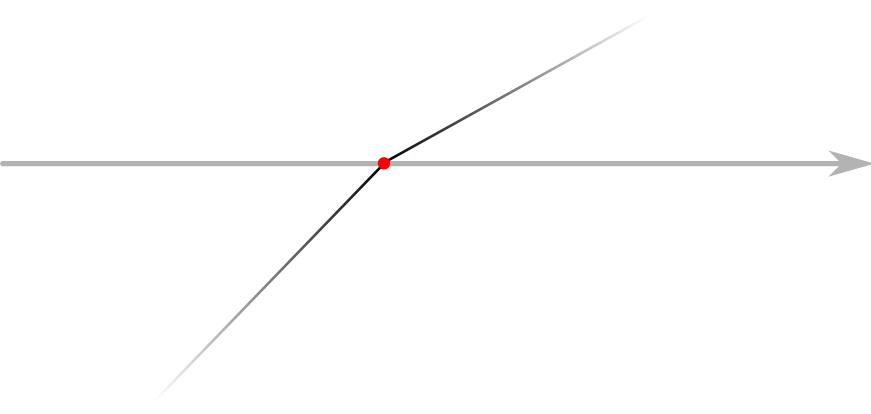
\includegraphics[scale=0.8]{./figuras/w_2.png}
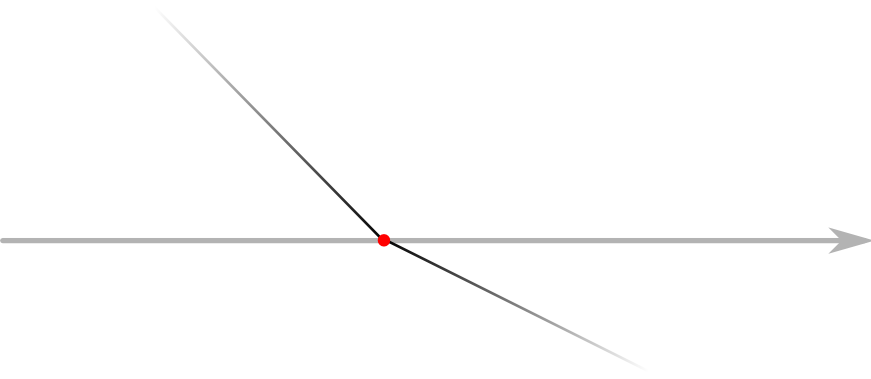
\includegraphics[scale=0.8]{./figuras/w_3.png}
\end{figure}

Intuitivamente, estos casos abren (primer figura) o cierran (segunda figura)
el polígono, por lo que debe contarse un cruce.

\begin{figure}[H]
\centering
\label{w_4y5}
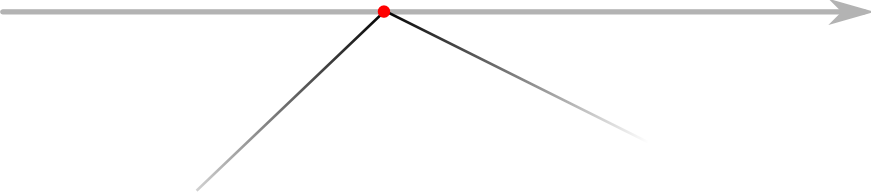
\includegraphics[scale=0.8]{./figuras/w_4.png}
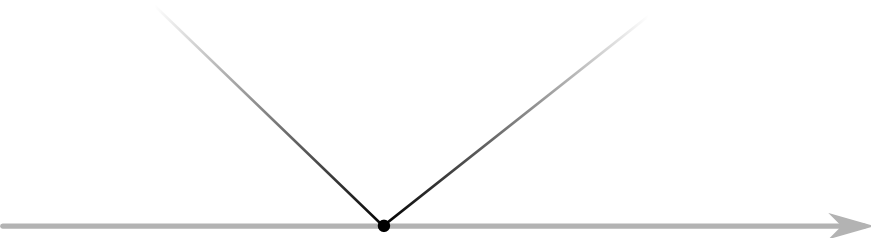
\includegraphics[scale=0.8]{./figuras/w_5.png}
\end{figure}

Intuitivamente, estos casos cierran y vuelven a abrir el polígono, por lo que debe mantener la paridad de
la cantidad de cruces. Si los lados del polígono que tienen este vértice como extremo tienen el otro extremo
por debajo de la recta, la cantidad de cruces contados son 2 (uno por cada segmento), por lo que la paridad se
mantiene. Si los lados tienen el otro extremo por encima de la recta, no se cuentan cruces (pues no cumple
la condición).
\end{itemize}

\subsection*{Detalles de Implementación}

Se implementó la clase \textbf{Desnivel}, que representa los polígonos según su cruce con el eje $X$.
Contiene dos números reales $x_1,x_2$ y un entero $altura$, que es la altura de las curvas de altura
del polígono.

Se implementó un método \textbf{contenido}, que dados dos Desniveles $a$ y $b$ verifica si
$b.x1 < a.x1 \wedge a.x2 < b.x2$.

El conjunto de polígonos que contienen solamente a Alice y solamente a Bob se
implementaron con dos vectores de desniveles. Se los ordena con el algoritmo
$quicksort$, que utiliza como condición el método \textbf{contenido}.

\subsection*{Pseudocódigo}

\begin{algorithm}[H]
\linesnumbered
\caption{walk($poligonos$)}
\Input{polígonos que forman las curvas de nivel del escenario}
\vspace{0.4cm}
\For{cada polígono} {
    \For{cada lado del polígono} {
        \If{cumple la condición de cruce con el eje $X$} {
            \If{el cruce es a la izq de Alice} {
                $cruceIzqAlice \gets$ cruce del segmento con el eje $X$
                
                $crucesIzqAlice++$
            }
            \If{el cruce es en el medio de Alice y Bob} {
                $cruceDerAlice \gets$ cruce del segmento con el eje $X$
                
                $cruceIzqBob \gets$ cruce del segmento con el eje $X$
                
                $crucesMedio++$
            }
            \If{el cruce es a la derecha de Bob} {
                $cruceDerBob \gets$ cruce del segmento con el eje $X$
            }
        }
    }
    
    \If{el polígono contiene a Alice y no a Bob} {
        $poligonosAlice \gets$ agregar $<cruceIzqAlice, cruceDerAlice, poligono.altura>$
    }
    \If{el polígono contiene a Bob y no a Alice} {
        $poligonosBob \gets$ agregar $<cruceIzqBob, cruceDerBob, poligono.altura>$
    }
}

calcularAlturaSubidaYBajada( poligonosAlice, poligonosBob )
\end{algorithm}

\begin{algorithm}[H]
\linesnumbered
\caption{calcularAlturaSubidaYBajada($poligonosAlice, poligonosBob$)}
\Input{vectores de pares que representan los poligonos que contienen solamente a Alice y los que contienen
solamente a Bob}
\vspace{0.4cm}

ordenar las secuencias poligonosAlice y poligonosBob por contención

$alturaSubida \gets 0$

$alturaBajada \gets 0$

\If{existe algún polígono que contenga a Alice} {
    $ultimaAltura \gets$ altura de $poligonosAlice.primero$
    
    \For{cada par $p$ en poligonosAlice despues del primero} {
        \If{$p.h < ultimaAltura$} {
            $alturaBajada \gets alturaBajada + ultimaAltura - p.h$
        }
        \Else {
            $alturaSubida \gets p.h - ultimaAltura$
        }
        $ultimaAltura \gets p.h$
    }
}

\If{existe algún polígono que contenga a Bob} {
    \If{no existe polígono que contenga a Alice} {
        $ultimaAltura \gets$ altura de $poligonosBob.primero$
        $poligonosBob \gets$ sacar primer elemento de la secuencia
    }
    \For{cada par $p$ en poligonosBob desde el último al primero} {
        \If{$p.h < ultimaAltura$} {
            $alturaBajada \gets alturaBajada + ultimaAltura - p.h$
        }\Else {
            $alturaSubida \gets p.h - ultimaAltura$
        }
        $ultimaAltura \gets p.h$
    }
}

imprimir alturaSubida alturaBajada
\end{algorithm}

\subsection*{Análisis de complejidad}

\textbf{calcularAlturaSubidaYBajada:}

La primer línea realiza un ordenamiento de dos vectores. En peor caso esta línea tiene complejidad
$O(max(a,b)^2)$, siendo $a$ la cantidad de elementos del vector poligonosAlice, y $b$ la cantidad de
elementos del vector polígonosBob. El caso promedio de esta línea es $O(max(a,b)*log(max(a,b)))$

Las líneas 2 hasta la 5 tienen costo constante, pues se trata de consultas y asignaciones a variables
resolubles en tiempo constante, al igual que el cuerpo del ciclo de la línea 6.
Dicho ciclo se ejecuta a lo sumo $a-1$ veces, por lo tanto las líneas 4 a 15 tienen
complejidad $O(a)$.

Las líneas 16 a 29 tienen costo constante, pues se trata de consultas y asignaciones a variables
resolubles en tiempo constante, al igual que el cuerpo del ciclo de la línea 20. Este ciclo
se ejecuta a lo sumo $b-1$ veces, por lo que el bloque de las líneas 16 a 30 tiene complejidad $O(b)$.

La línea 30 tiene complejidad constante.

Por lo tanto el algoritmo {\bf calcularAlturaSubidaYBajada} tiene complejidad
$O(max(a,b)^2)$ en peor caso, y $O(max(a,b)*log(max(a,b)))$ en caso promedio.\\


\textbf{walk:}

Las líneas 3 a 16 tienen costo constante, pues se trata de consultas y
asignaciones a variables resolubles en tiempo constante.

El ciclo de la línea 2 se ejecuta a lo sumo $P_i+1$ veces, siendo $P_i$ la
cantidad de vértices del polígono $i$. Por tanto el ciclo tiene complejidad $O(P_i)$.

Las líneas 18 a 23 tienen costo constante, ya que se trata de consultas y
{\sl push} de un elemento al final de un vector.

El ciclo de la línea 1 se ejecuta a lo sumo $N$ veces (con $N$ la cantidad de polígonos).
Por tanto el ciclo principal tiene complejidad $O(Nmax\{P_i\})$.

La línea 25 llama a {\bf calcularAlturaSubidaYBajada}, que tiene complejidad
$O(max(a,b)^2)$ en peor caso y $O(max(a,b)*log(max(a,b)))$ en caso promedio,
como vimos anteriormente. El peor caso en este problema para este algoritmo
sería que todos los polígonos contengan a Alice o a Bob, por lo que $max(a,b)
= N$, y en caso promedio sería $max(a,b) = \frac{N}{2}\pm 1$ (según N sea par o impar),
lo que hace la complejidad $O(N^2)$ en peor caso y $O(N\log N)$ en caso
promedio.\\

Concluímos que nuestro algoritmo {\bf walk} tiene complejidad $O(Nmax(P_i)+N^2)$ en peor caso,
y $O(Nmax(P_i) + N\log N)$ en caso promedio, siendo $N$ la cantidad de polígonos y
$P_i$ la cantidad de lados del polígono $i$.

\newpage
\section*{4289 -- ``Disgruntled Judge''}
\subsection*{Problema y solución}

El problema consiste en encontrar un valor entero para $a$ y $b$ dados $T$
valores de entrada. A partir de estos dos valores se pueden generar los $T$
valores de salida siguiendo la ecuación de congruencia, definida de la
siguiente manera:

FIXME: ¿= o $\equiv$?:
$$X_k = aX_{k-1} + b\ (10001)$$

Como los valores de entrada están intercalados con los de salida y definidos
sobre los impares, el problema se transforma en hallar el par $(a,b)$ que
resuelve las $T$ ecuaciones, de la siguiente forma:

FIXME: ¿*+?:
$$X_k \equiv (aX_{k-2} + b) * + b\ (10001)$$

Como 10001 no es un número primo ($10001 = 137\times 73$), esto se puede
llevar, por el teorema chino del resto, a hallar el par $(a,b)$ que cumple con
las siguientes 2 ecuaciones:

FIXME: ¿*+?: 
$$X_k \equiv (aX_{k-2} + b) * + b\ (137)$$
$$X_k \equiv (aX_{k-2} + b) * + b\ (73)$$


\subsection*{Detalles de Implementación}

Para hallar la solución utilizamos una versión simple del algoritmo que busca
en el espacio del anillo de $Z-10001$ el par de valores que hacen verdaderas
las $T$ ecuaciones. Como puede existir más de una solución, tomamos el primer
par válido que cumpla para computar el output. Para agilizar los cálculos, a
medida que ingresamos el input de los valores precalculamos el módulo 73 y 137
de esos valores, con el fin de que los factores utilizados en las cuentas sean
más pequeños. (FIXME, refacotrizar:) Además buscamos una manera eficiente para
calcular el módulo del valor de la iteración actual. Luego resta verificar que
los valores testeados en la iteración sean el par de valores buscados, y
calcular a partir de ellos los valores de salida.


\subsection*{Análisis de complejidad}

Esta versión del algoritmo recorre de manera lineal para $a$ y $b$ los valores
posibles módulo 10001, y luego verifica para cada par que efectivamente cumpla
las $T$ ecuaciones de congruencia. El orden final del algoritmo es de
$O(TN^2)$, donde $T$ es el número de casos de test y $N$ es el valor del módulo.


\newpage
\bibliographystyle{acm}
\bibliography{citas}

\end{document}
